\chapter{Einleitung}
\label{chap:einleitung}

Dieses Dokument dient einerseites zur Illustration der \LaTeX{} Vorlage anhand des Corporate Designs\index{Corporate Design} der Berner Fachhochschule\index{Berner Fachhochschule} und andererseits als Anleitung für deren Verwendung. Dabei wird vorausgesetzt, dass der Benutzer bereits Erfahrungen mit \LaTeX{} besitzt oder gewillt ist, sich während der Benutzung in das Thema einzuarbeiten. Im Quellenverzeichnis sind einige nützliche Einträge zu diversen Büchern und Dokumenten im Internet über \LaTeX{} zu finden.

% Einträge im Verzeichnis erscheinen lassen ohne hier eine Referenz einzufügen
\nocite{kopka:band1}
\nocite{raichle:bibtex_programmierung}
\nocite{MiKTeX}
\nocite{KOMA}
\nocite{TeXnicCenter}
\nocite{Marti06}
\nocite{Erbsland08}
\nocite{juergens:einfuehrung}
\nocite{juergens:fortgeschritten}

\section{Dokumentaufbau}
\label{sec:einleitung_aufbau}

Das vorliegende Dokument ist so aufgebaut wie die Dokumentation einer Projektarbeit oder Thesis\index{Thesis}. Im Kapitel \ref{chap:anleitungen} werden die verwendeten Pakete kurz erklärt und Hinweise gegeben, wie die Bibliographie und das Glossar zu verwenden sind. Kapitel \ref{chap:satzspiegeltest} stellt ein reines Beispielkapitel dar, um den Satzspiegel zu prüfen.

In Abbildung \ref{fig:datei_struktur} ist die Dateistruktur dieses Template dargestellt.

\begin{figure}[H]
	\centering
		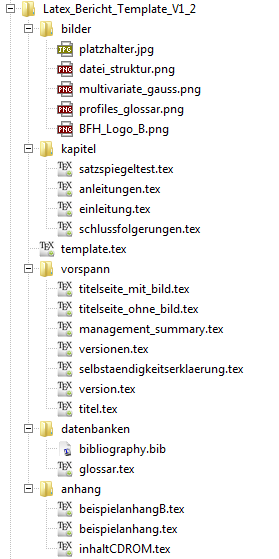
\includegraphics[scale=0.85]{bilder/datei_struktur.png}
	\caption{Dateistruktur}
	\label{fig:datei_struktur}
\end{figure}

\section{Kontakt}
\label{sec:einleitung_kontakt}

Die Hersteller dieser Vorlage sind natürlich froh um Verbesserungsvorschläge jeder Art. Kapitel \ref{sec:einleitung_vorschlaege} enthält mögliche Verbesserungsvorschläge\index{Verbesserungsvorschläge}.

\begin{table}[H]
	\centering
		\begin{tabular}{lll} \toprule
			\textbf{Vorname Name} & \textbf{E-Mail} & \textbf{Funktion} \\ \midrule
			Alfred Kaufmann & alfred.kaufmann@bfh.ch & Auftraggeber, Projektleitung, Ergänzungen \\ \midrule
			Fritz Dellsperger & in Pension & Tipps zur Struktur und Layout \\ \midrule
			David Burri & ausgetreten & Erstellung der Vorlage \\ \bottomrule
		\end{tabular}
	\caption{Kontaktpersonen}
	\label{tab:kontaktpersonen}
\end{table}


\section{Verbesserungsvorschläge}
\label{sec:einleitung_vorschlaege}

\begin{itemize}
	\item Erstellen eines eigenen BFH Style-Files
	\item Vorlage für die Präsentationserstellung mit \LaTeX{}
\end{itemize}


